\section{Basisstation} \label{sec:basestation}

% Het basisstation is gemaakt om data weer te geven aan de gebruiker en ook om het communicatiesysteem te kunnen debuggen.
% \subsubsection{Functionele blokken}

% \paragraph{Callback functies}
% De gehele interface is zo modulair mogelijk opgebouwd. De windows bestaan uit elementen die je kan aanmaken met de volgende functie.
% In deze functie kan je als argument 2 andere functies meegeven, een clickCallback die de touch coördinaten mee krijgt en een initCallback die de window meekrijgt zodat je erin de visuele ncruses functies kan oproepen. 
% \begin{lstlisting}[caption={ScreenElement},captionpos=b,label={lst:ScreenELement},style=c]
% static screenElement_t addScreenElement(
%     screen_t *screen, uint32_t startRow,
%     uint32_t startCol, uint8_t height, uint8_t width,
%     void (*clickCallback)(uint32_t, uint32_t),
%     void (*initCallback)(WINDOW *win)
% ); return res - offset;
% \end{lstlisting}

Het basisstation is bedoelt om de data van de sensoren weer te geven aan de gebruiker. Ook kan het gebruikt worden om het sensornetwerk te debuggen, doordat het live diagnostische data over het netwerk op het scherm kan weergeven. Het basisstation bestaat uit een Raspberry PI met een touchscreen display. De PI is verbonden met een XMega die dient als node in het netwerk.

\subsection{Interface}
De interface van het basisstation bestaat uit 2 verschillende schermen: het debug scherm en het gebruikersscherm.

\subsubsection*{Debug scherm}
Het debug scherm is nuttig om te zien of nodes in het netwerk goed werken. 
Het gehele scherm wordt gebruikt verschillende data te laten zien. 
\begin{figure}[ht]
    \centering
    \includegraphics*[width=0.8\textwidth]{img/basestationInterface.png}
    \caption{Debug scherm op de 7 inch PI scherm.}
    \label{fig:debugSchermScreenshot}
\end{figure}

\begin{figure}[ht]
    \centering
    \includegraphics*[width=0.8\textwidth]{img/debugScreenExplain.pdf}
    \caption{De verschillende onderdelen van het debug scherm}
    \label{fig:debugSchermUitleg}
\end{figure}
Het debug scherm is bedoeld om informatie over het netwerk weer te geven. Het bestaat uit verschillende onderdelen, die zijn opgedeeld in vensters. Een schematische weergave van deze vensters is te zien in \autoref{fig:debugSchermUitleg}.

Het Broadcasts venster toont de constante stroom van broadcast-berichten die de basisstation node ontvangt. De broadcasts worden getoond als hexadecimale waardes. Door de kleine afmetingen van het scherm (30 rijen bij 100 kolommen aan karakters), zijn de waardes niet met spaties opgesplitst, maar met twee duidelijk verschillende en leesbare kleuren. Wanneer het venster vol staat met data, scrolt hij voor elke broadcast telkens een regel verder.

Het Relays \& Payloads venster toont alle ontvangen directe berichten. Dit is inclusief doorstuurberichten die niet voor het basisstation bedoeld zijn. Om hier onderscheid in te maken worden de berichten die wel voor het basisstation bedoeld zijn lichter geprint. Onder de rij met bytes worden de corresponderende ASCII karakters geprint voor elke byte die een geldig ASCII karakter heeft. Dit wordt gedaan om berichten die tekstuele data bevatten te kunnen ontcijferen.

Het Buttons venster bevat de coördinaten van de laatste aanraking op het touchscreen, en twee knoppen. Eén van de knoppen kan gebruikt worden om de Raspberry PI veilig af te sluiten, de andere kan gebruikt worden om te schakelen tussen het debug scherm en het normale scherm.

Het Friends venster bevat de lijst van vriendjes die de basisstation node kent. Elke regel in het venster toont de data van één vriendje. Als er op de regel getikt wordt verschijnt er een prompt die vraagt of er een bericht gestuurd moet worden naar de node waar op getikt is, zoals te zien in \autoref{fig:friendSend}. Als er vervolgens op ``yes'' getikt wordt, stuurt het basisstation een standaard bericht naar de geselecteerde node.

\begin{figure}[ht]
    \centering
    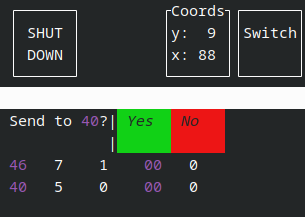
\includegraphics[width=0.3\textwidth]{img/prompt.png}
    \caption{Verstuur prompt op het debug scherm.}
    \label{fig:friendSend}
\end{figure}

Het Data venster toont de actuele sensordata. Wanneer er nog geen data ontvangen is van een bepaalde sensor, staat er ``measuring''.

\subsubsection*{Gebruikersscherm}
Het gebruikersscherm is het scherm dat door de gebruiker gezien hoort te worden. Hierop is alle sensor data beschikbaar, net als het data venster in de debug interface. Ook is er een plaats waar de metaconclusies verschijnen.




\subsection{Software}
De code van de interface gebruikt een modulair systeem om aanpassingen zo makkelijk mogelijk te maken. De twee schermen, het debug scherm en het gebruikersscherm, zijn gedefinieerd met een scherm datatype.
Deze `schermen' bevatten vervolgens een array van `scherm elementen'.

\begin{minipage}{\textwidth}
    \begin{lstlisting}[caption={Het datatype van de schermen},captionpos=b,label={lst:screen_t},style=c,xleftmargin=.\textwidth,xrightmargin=.\textwidth]
typedef struct {
    uint8_t elementCount;
    screenElement_t *elements;
} screen_t;
    \end{lstlisting}
\end{minipage}

Een scherm element moet een aantal dingen kunnen opslaan. Elk scherm element heeft een ncurses window nodig om naar de interface te kunnen printen. Deze bevat ook gelijk de dimensies en de positie van het element.
Daarnaast is het handig als het mogelijk is om op het touchscreen een scherm element aan te kunnen tikken. Hierdoor heeft elk scherm element een functie pointer, die uitgevoerd wordt wanneer er op het element getikt wordt. Omdat een bepaalt element misschien wilt weten waar er precies getikt is, accepteert deze functie 2 coördinaten als argumenten. Als het scherm element geen tik functie nodig heeft, kan deze naar een null pointer gezet worden. Als laatste moet elk scherm element opnieuw naar de interface getekend kunnen worden, wanneer er van scherm gewisseld wordt. Hiervoor is een initialisatie functie pointer toegevoegd. Deze wordt uitgevoerd wanneer het scherm waar het element in zit geïnitialiseerd wordt.

\begin{lstlisting}[caption={Het datatype van de scherm elementen},captionpos=b,label={lst:screenElement_t},style=c,xleftmargin=.\textwidth,xrightmargin=.\textwidth]
typedef struct {
    WINDOW *window;
    void (*tap)(uint32_t col, uint32_t row);
    void (*initialize)(WINDOW *win);
} screenElement_t;    
\end{lstlisting}

\subsubsection*{Communicatie met de XMega}

De Raspberry PI communiceert met de XMega met een UART/USB connectie. De XMega stuurt continu diagnostische data over het netwerk naar de PI. Deze moet de PI dan vervolgens kunnen interpreteren. Aangezien een PI geen verbinding kan maken met een microcontroller die nog niet is aangesloten, is het wenselijk om de XMega te hebben aangesloten voordat het interface programma op de PI gestart wordt. Wanneer het programma opstart stuurt de PI een opstartbyte naar de XMega, en wacht totdat deze reageert. De XMega gaat pas data sturen wanneer deze de opstartbyte heeft ontvangen. Op deze manier weet de PI altijd wat de eerste byte is die de XMega heeft gestuurd. Wanneer het programma afgesloten wordt stuurt de PI ook een afsluit byte naar de XMega, zodat deze stopt met data sturen.

Er zijn 5 verschillende soorten berichten die de XMega kan sturen. De PI moet kunnen weten met welk soort bericht hij te maken heeft, dus is er een systeem bedacht met identificerende bytes. Elk bericht dat de XMega stuurt begint met een identificerende byte. Deze byte wordt de `protocol byte' genoemd, en geeft aan op welke manier de PI de data erna moet parsen. Hier volgt een korte beschrijving van elk van de protocollen:

\begin{description}

\item[ID protocol] De PI moet weten welk ID zijn node heeft. Hiervoor is het ID protocol gemaakt. Het enige wat het ID protocol hoeft te sturen is het ID, dus het is een erg simpel protocol.\\
\begin{tabular}{ |c|c| } 
    \hline
    Protocol Byte & Node ID \\ 
    \hline
\end{tabular}


\item[Vriendenlijst protocol] De vriendenlijst wordt opgestuurd met een header gevolgd door een herhalend deel. Het herhalende deel bevat alle informatie van één vriendje, en wordt voor elk vriendje in de lijst herhaald. De Pi weet hoeveel van deze herhalingen er gelezen moeten worden door een byte in de header die aangeeft hoeveel vriendjes er zijn verstuurd.\\
\begin{tabular}{ |c|c||c|c|c|c|c| } 
    \hline
    Protocol Byte & Aantal vriendjes & Vriend ID & Hops & Via & Trust & Active \\ 
    \hline
\end{tabular}

\item[Payload protocol] Ontvangen payloads worden doorgestuurd door middel van het payload protocol. De PI kent zijn eigen ID al, dus deze hoeft niet meegestuurd te worden.\\
\begin{tabular}{ |c|c| } 
    \hline
    Protocol Byte & Payload (31 bytes) \\ 
    \hline
\end{tabular}

\item[Doorstuur protocol] Een doorgestuurde packet wordt met een apart protocol gestuurd. Dit is zodat de PI heel makkelijk onderscheid kan maken tussen een doorgestuurd bericht en een payload die voor het basisstation bedoeld is.\\
\begin{tabular}{ |c|c| } 
    \hline
    Protocol Byte & Packet (32 bytes) \\ 
    \hline
\end{tabular}


\item[Broadcast protocol] Als laatste moet de PI de binnenkomende broadcasts kunnen laten zien. Deze worden doorgestuurd met het broadcast protocol. Het broadcast protocol is in principe gewoon het doorstuur protocol met een andere protocol byte, zodat de PI weet dat het gaat om een broadcast in plaats van een doorgestuurd bericht.\\
\begin{tabular}{ |c|c| } 
    \hline
    Protocol Byte & Packet (32 bytes) \\ 
    \hline
\end{tabular}

\end{description}

% Zoals te zien in \autoref{fig:debugSchermScreenshot}, is het scherm opgedeeld in 5 delen. Links boven kan je alle broadcast berichten zien die de basisstation ontvangt. 
% Links onder in het scherm zie je alle privé relays en payloads die via de basisstation. Dan kijken we rechts boven, hier zitten 2 knoppen en een touch coords window. Een van de knoppen zet de PI veilig uit. De andere switcht naar de User data scherm die beschreven wordt in \autoref{ch:userParagraph}.
% De coords geven aan waar de laatste touch was op het scherm in rijen en kolommen. In totaal zijn er 30 rijen op Y as en 100 kolommen op de X as. Dit was een van de eerste windows die we hadden toegevoegd en heeft veel geholpen met positioneren van alle objecten op het scherm.
% Rechts midden kan je een vriendenlijst zien die vanuit de basisstation xMega wordt weergegeven. Daaronder zien we een `data from sensor nodes', dit is een window die onze dummy data laat zien vanuit de potmeters van andere nodes. 
% \subsubsection{User data scherm}\label{ch:userParagraph}
% Als je switcht naar de user data scherm dan krijg je de `data from sensor nodes' te zien. Dit is een window precies zoals hij te zien in de debug window.
% Ook komt er nog een meta conclusies als de data vanuit de sensoren boven een grens komt. Dan zegt de interface `Je moet een raam open doen, de luchtkwaliteit is slecht". Dit is nog iets wat verbeterd moet worden, onze user scherm is heel erg kaal.